\section{Incident Source Conditions}
Primarily there are two kinds of sources in FDTD: point sources and plane wave sources.

Point source can be classified as hard source or soft source. If the source value is directly assigned to the certain
point, this is referred to as a hard source. Oppositely, it can be called a soft source if the source value is added to
the field at that point. A hard source would lead to some reflection between certain points and adjacent points and a
soft source allows wave just pass through. Point source is not common used in 2D and 3D simulation but play a important
role on constructing plane wave source conditions.

For investigating nano structures, it's often of interest to impinge plane wave source upon structures and measure
transmission and reflection. The calculation of radar cross section also deals with plane wave. Total Field / Scatter
Field (TFSF) is a technique to to simulate a plane wave by dividing problem space into Totol Field region and Scatter
Field region(Fig.\ref{fig:tfsf}).

\begin{center}\label{fig:tfsf}
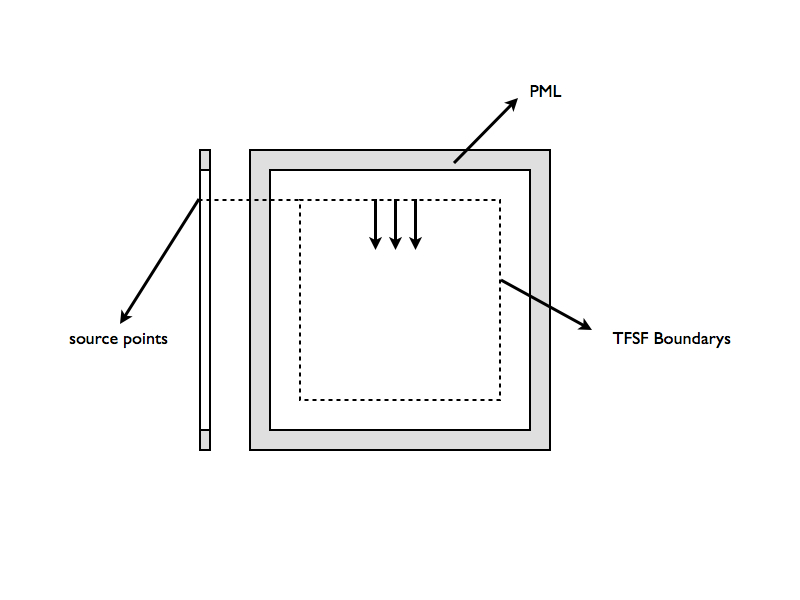
\includegraphics[scale=0.5]{images/tfsf.jpg}
\end{center}

The TFSF formulas can be observed through complete update equation and totol/scatter field theory

\begin{displaymath}
  E_{total}=E_{scatter}+E_{incident}
\end{displaymath}
\begin{displaymath}
  H_{total}=H_{scatter}+H_{incident}  
\end{displaymath}


The Y incident plane wave of TM polarization can be create through following formulas

integrate $D_z$ and $B_x$ at $j=ja$ and $j=jb$
\begin{displaymath}
  D_z|_{i,ja} = D_z|_{i,ja} + 0.5 \cdot H_{inc}|_{ja-\frac{1}{2}}
\end{displaymath}
\begin{displaymath}
  D_z|_{i,jb} = D_z|_{i,jb} - 0.5 \cdot H_{inc}|_{jb+\frac{1}{2}}  
\end{displaymath}
\begin{displaymath}
  B_x|_{i,ja-\frac{1}{2}}=B_x|_{i,ja-\frac{1}{2}}+0.5 \cdot E_{inc}|_{ja}
\end{displaymath}
\begin{displaymath}
  B_x|_{i,jb+\frac{1}{2}}=B_x|_{i,jb+\frac{1}{2}}-0.5 \cdot E_{inc}|_{jb}
\end{displaymath}
$B_y$ should be integrated at the intefate at $i=ia$ and $i=ib$
\begin{displaymath}
  B_y|_{ia-\frac{1}{2},ja:jb}=B_y|_{ia-\frac{1}{2},ja:jb}-0.5 \cdot E_{inc}|_{ja:jb}
\end{displaymath}
\begin{displaymath}
  B_y|_{ib+\frac{1}{2},ja:jb}=B_y|_{ib+\frac{1}{2},ja:jb}+0.5 \cdot E_{inc}|_{ja:jb}
\end{displaymath}






